\section{Sviluppatori}
\subsection{UC 4.1 - Visualizzazione elenco frasi}
\begin{itemize}
\item[•]\textbf{Attori}: Sviluppatore;
\item[•]\textbf{Descrizione}: Lo sviluppatore visualizza un elenco di frasi accompagnate dalla data di creazione e dall’autore ordinate cronologicamente;
\item[•]\textbf{Precondizione}:  L'amministratore ha approvato l’utenza dello sviluppatore e lo sviluppatore si è autenticato nel sistema.
\item[•]\textbf{Postcondizione}: 
\item[•]\textbf{Flusso degli eventi principale}: Lo sviluppatore ha selezionato la voce relativa alla pagina contenente l’elenco delle frasi e ne visualizza il contenuto; 
\end{itemize}
\subsection{UC 4.2 - Filtraggio dei dati}
%\begin{figure}[H]
%\centering
%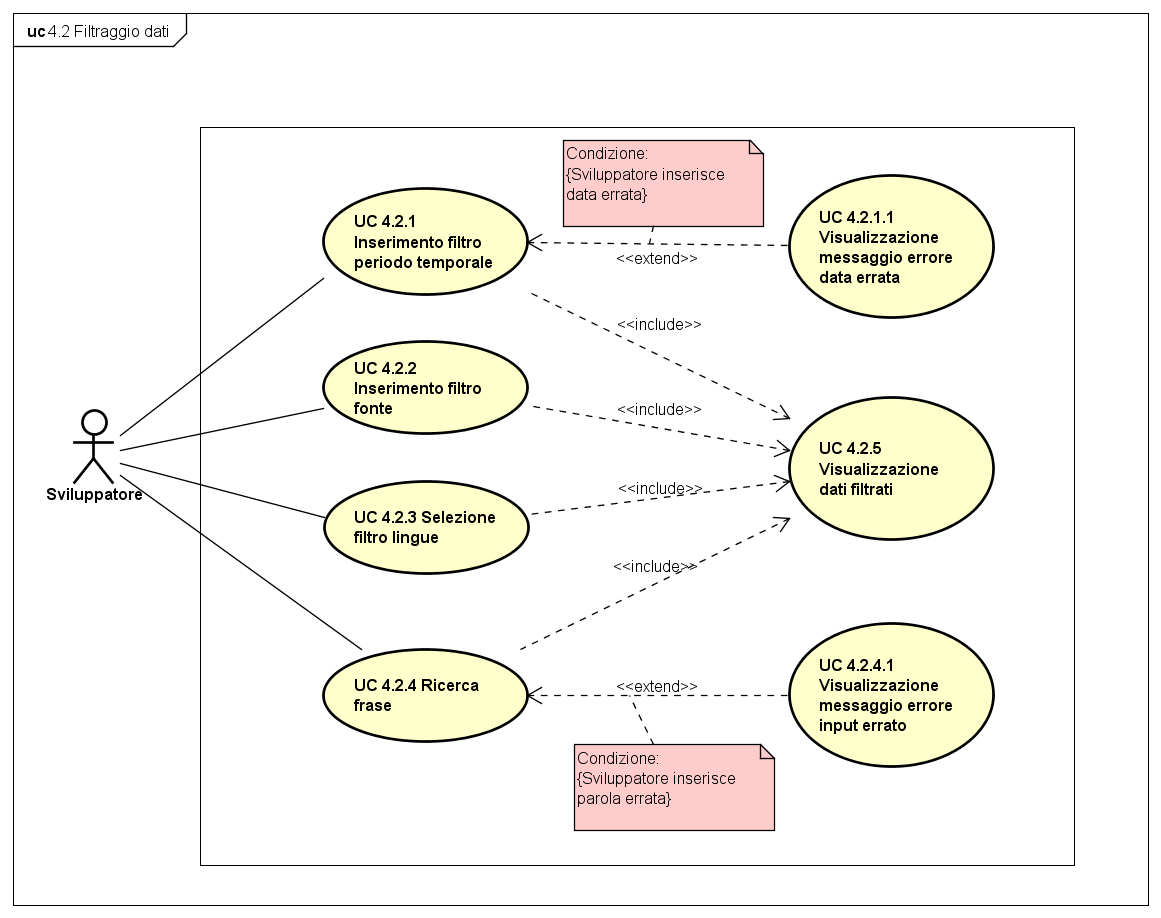
\includegraphics[width=17cm]{img/UC420.png} 
%\caption{Caso d'uso 4.2}
%\label{fig:420}   %non capisco cosa sia label 
%\end{figure}
\begin{itemize}
\item[•]\textbf{Attori}: Sviluppatore;
\item[•]\textbf{Descrizione}: Lo sviluppatore applica dei filtri ai dati, ottenendo solo quelli d’interesse;
\item[•]\textbf{Precondizione}: Lo sviluppatore visualizza le proposizioni in ordine cronologico;
\item[•]\textbf{Postcondizione}: Lo sviluppatore visualizza i dati che rispettano i filtri scelti;
\item[•]\textbf{Flusso degli eventi principale}:
\begin{enumerate}
\item UC 4.2.1 Inserimento filtro periodo temporale;
\item UC 4.2.2 Inserimento filtro fonte\ped{G};
\item UC 4.2.3 Visualizzazione storico frase;
\item UC 4.2.4 Selezione filtro lingue;
\item UC 4.2.5 Ricerca parole chiave;
\end{enumerate}
\end{itemize}
\subsubsection{UC 4.2.1 - Inserimento filtro periodo temporale}